\subsection{Opgave 51}

Nedenfor ses grafen for en funktion f.

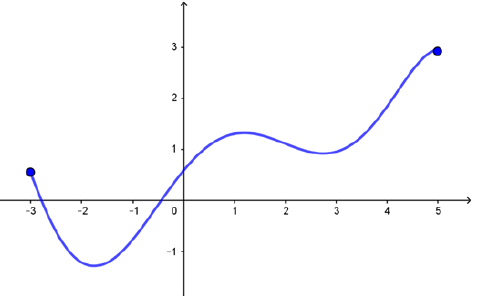
\includegraphics[width=8cm]{Opgave_51-56/Opgave_51/51.png}

Benyt grafen til at bestemme fortegnet på $f'(-1)$.

\ans

Har vi en graf $f(x)$ så fortæller fortegnet på $f'(x)$ i en bestemt x værdi om vores funktion $f(x)$
har en positiv hældning, altså at den er voksende eller at den har en negativ hældning, altså at den er aftagende.

Kigger vi på grafen hvor $x = -1$ kan vi se at $f(x)$ er voksende hvilket betyder at fortegnet for $f'(-1)$ er positivt.



